\chapter{Kostenberechnung}
\label{Kostenberechnung}

Die Kostenfunktion stellt in jedem VRP und dessen Ablegern eine Kernkomponente dar. 
Diese muss an das Problem angepasst werden und ist somit problem- und zielspezifisch. 
Mit dieser Funktion wird definiert wie und was optimiert werden soll. 
Zum Beispiel kann diese so ausgelegt sein, dass die Strecke oder Fahrzeit minimal sein soll oder beides gemeinsam. 
Im weiteren Verlauf dieses Kapitels wird auf einige Eigenschaften der Kostenfunktion für den Savings-Algorithmus eingegangen.  

\section{Distanz-Basierend}

Rein auf Distanz-Basierende-Kostenfunktionen bringen meist nicht das gewünschte Ergebnis zu Tage. 
Dies lässt sich auf die Einschränkung der vorhandenen Daten zurückführen. 
Alle Ergebnisse basieren dabei rein auf den Distanzen, welche gefahren werden. 
In diesem Fall könnte ein Kunde einige wenige Kilometer entfernt sein, direkt aber nur über einen Feldweg. 
Dies würde zu einer kurzen Distanz führen ohne die Beschaffenheit der Strecke und der dabei benötigten Zeit zu berücksichtigen. 
Sollte trotzdem nur die Distanz zur Verfügung stehen, so ist dies besser als überhaupt keine Informationen zu haben. 

\noindent
Die Berechnung für die Ersparnis im SA ist in der Gleichung \ref{eq:savingbase} zu finden. 
Dabei stellen die Punkte \textit{A} und \textit{B} zwei Kunden dar und \textit{DE} das Depot, von welchem aus losgefahren wird. 
Die Variable \textit{dis} repräsentiert die Distanzmatrix, welche alle Distanzen zwischen den Punkten beinhaltet. 
Die Ersparnis ist hierbei definiert als das, was eingespart wird, wenn zwischen Kunde \textit{A} und \textit{B} nicht zum Depot zurückgekehrt, sondern direkt von \textit{A} nach \textit{B} gefahren wird \cite{clarke1964scheduling}. 
\begin{equation}
sav_{a,b} := dis_{a,z} + dis_{z,b} - dis_{a,b}
\label{eq:savingbase}
\end{equation}

\noindent
In der Abbildung \ref{fig:simpleNetwork} ist ein einfaches Netzwerk mit Kunden und einem Depot abgebildet. 
Die Abkürzung \textit{AB} steht in diesem Beispiel für Autobahn, \textit{LS} für Landstraße und \textit{FW} für Feldweg. 
Wie in dieser Abbildung festgestellt werden kann, existieren zwei Kanten mit einem Feldweg und eine mit einer Autobahn. 
An diesem Beispiel lässt sich erkennen, dass die Beschaffenheit des Fahrwegs ignoriert und vernachlässigt wird. 
In Tabelle \ref{tab:distSavings} befinden sich die Ergebnisse der Ersparnisse zu Beginn des Savings-Algorithmus nach der Initialisierung. 
Im Gesamten lässt sich hier erkennen, dass lange Strecken bevorzugt werden. 
In diesem Fall würden zuerst die Routen \textit{A - B} oder \textit{D - E} zusammengefügt werden, abhängig von der Sortierung der Savings-Liste. 
\begin{figure}
\centering
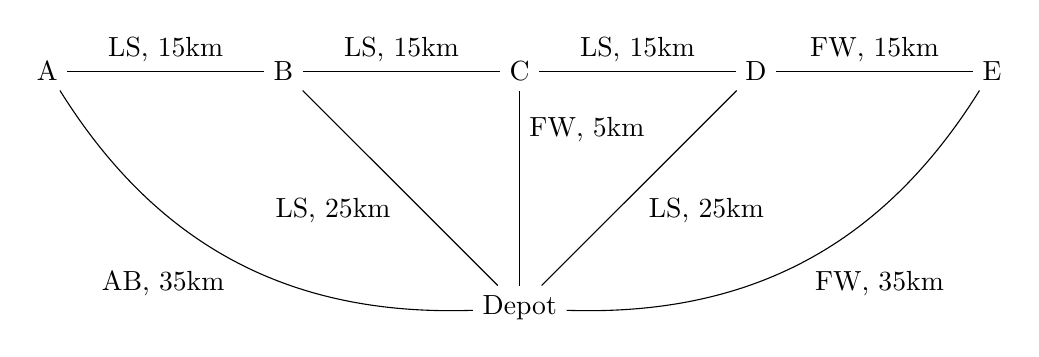
\begin{tikzpicture}[auto, node distance=3cm]
	%\tikzstyle{every node}=[draw,shape=circle];
	
	\node (a) {A};
	
	\node (b) [right of=a] {B};
	
	\node (c) [right of=b] {C};
	
	\node (d) [right of=c] {D};
	
	\node (e) [right of=d] {E};
	
	\node (de) [below of=c] {Depot};
	
	\path 	(de) 	edge [bend left] node {AB, 35km} (a)
					edge node {LS, 25km} (b)
			 		edge node [right, pos=0.8] {FW, 5km} (c)
			 		edge node [below right] {LS, 25km} (d)
			 		edge [bend right] node [below right] {FW, 35km} (e)
			(a)		edge node {LS, 15km} (b)
			(c) 	edge node [above] {LS, 15km} (b)
			(d)		edge node [above] {LS, 15km} (c)
			(d)		edge node {FW, 15km} (e);
\end{tikzpicture}

	\caption{Ein einfaches Netzwerk mit $4$ Kunden und einem Depot}
	\label{fig:simpleNetwork}
\end{figure}
\begin{table}[htb]%[ht!]
\centering% NICHT \begin{center}
\begin{tabular}{p{3cm}|p{4cm}}
%\hline 
Route & Ersparnis \\ 
\hline 
A $\leftrightarrow$ B & $35 + 25 - 15 = 45$ \\ 
%\hline 
B $\leftrightarrow$ C & $25 + 5 - 15 = 15$ \\ 
%\hline 
C $\leftrightarrow$ D & $5 + 25 - 15 = 15$ \\ 
%\hline 
D $\leftrightarrow$ E & $25 + 35 - 15 = 45$ \\ 
%\hline 
\end{tabular} 
\caption{Aufschlüsselung der Ersparnisse anhand der Teilrouten zu Beginn der Optimierung}
\label{tab:distSavings}
\end{table}

\noindent
An diesem Beispiel lässt sich erkennen, dass die Beschaffenheit einer Straße ignoriert wird. 
Für den Algorithmus sieht dies so aus, als ob dies eine gute Kombination wäre.
Im Grund stimmt dies, zumal die Ersparnis größer ist. 

\section{Zeit-Basierend}

Zeit-Basierende-Kostenfunktionen beinhalten einen Vorteil gegenüber der Distanz-Basierten-Version, aber bergen auch Probleme. 
Der Vorteil der Zeitinformation liegt darin, dass die Beschaffenheit der Strecke versteckt mit einfließt. 
So wird auf einer Strecke mit Autobahn weniger Zeit benötigt, als auf derselben Distanz, aber mit Feldweg als Beschaffenheit. 

\noindent
Die Berechnung für die Ersparnis im Savings-Algorithmus ist in der Gleichung \ref{eq:savingbasezeit} zu finden. 
Dabei ist diese identisch mit der Gleichung aus \ref{eq:savingbase} mit dem Unterschied, dass hier eine Zeitmatrix \textit{time} verwendet wird. 
\begin{equation}
sav_{a,b} := time_{a,z} + time_{z,b} - time_{a,b}
\label{eq:savingbasezeit}
\end{equation}

\noindent
In Abbildung \ref{fig:simpleNetworkTime} befindet sich das gleiche Netzwerk aus \ref{fig:simpleNetwork}, aber mit Zeiten an den Kanten. 
Die Abkürzung \textit{AB} steht für Autobahn mit $130\,km/h$, \textit{LS} für Landstraße mit $100\,km/h$ und \textit{FW} für Feldweg mit $10\,km/h$. 
In der Tabelle \ref{tab:distSavingsZeit} befinden sich die Ergebnisse der Ersparnisse zu Beginn des Savings-Algorithmus nach der Initialisierung.
Erkennbar ist hier, dass nicht die Strecke mit der Autobahn bevorzugt wird, sondern der langsame Feldweg. 
Dieses Verhalten führt unweigerlich dazu, dass der Feldweg als erste Kombination verwendet wird. 
\begin{figure}
\centering
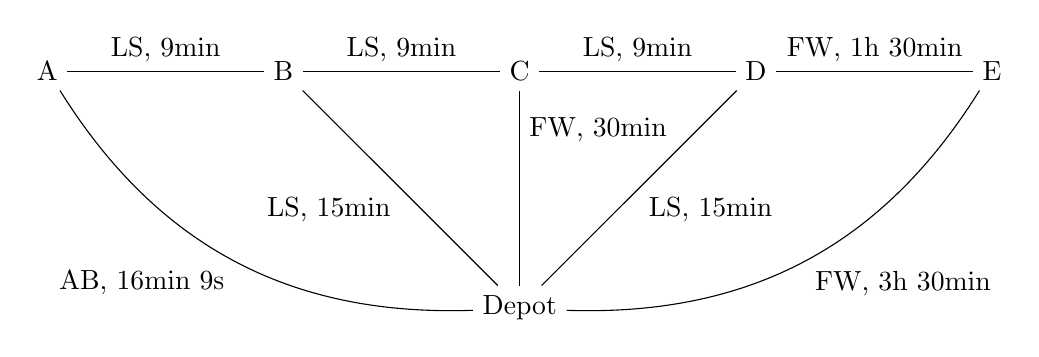
\begin{tikzpicture}[auto, node distance=3cm]
	%\tikzstyle{every node}=[draw,shape=circle];
	
	\node (a) {A};
	
	\node (b) [right of=a] {B};
	
	\node (c) [right of=b] {C};
	
	\node (d) [right of=c] {D};
	
	\node (e) [right of=d] {E};
	
	\node (de) [below of=c] {Depot};
	
%	\path 	(de) 	edge node {AB, 16min 9s} (a)
%					edge [bend left] node {LS, 15min} (b)
%			 		edge node {FW, 30min} (c)
%			 		edge [bend right] node {LS, 15min} (d)
%			 		edge node {FW, 3h 30min} (e)
%			(a)		edge [bend right] node {LS, 9min} (b)
%			(c) 	edge [bend right] node {LS, 9min} (b)
%			(d)		edge [bend right] node {LS, 9min} (c)
%			(d)		edge [bend right] node {FW, 9min} (e);
			
	\path 	(de) 	edge [bend left] node {AB, 16min 9s} (a)
					edge node {LS, 15min} (b)
			 		edge node [right, pos=0.8] {FW, 30min} (c)
			 		edge node [below right] {LS, 15min} (d)
			 		edge [bend right] node [below right] {FW, 3h 30min} (e)
			(a)		edge node {LS, 9min} (b)
			(c) 	edge node [above] {LS, 9min} (b)
			(d)		edge node [above] {LS, 9min} (c)
			(d)		edge node {FW, 1h 30min} (e);
\end{tikzpicture}

	\caption{Derselbe Graph aus \ref{fig:simpleNetwork} mit $4$ Kunden und einem Depot mit den benötigten Zeiten}
	\label{fig:simpleNetworkTime}
\end{figure}
\begin{table}[htb]%[ht!]
\centering% NICHT \begin{center}
\begin{tabular}{p{3cm}|p{4cm}}
%\hline 
Route & Ersparnis \\ 
\hline 
A $\leftrightarrow$ B & $16,15 + 15 - 9 = 22,15$ \\ 
%\hline 
B $\leftrightarrow$ C & $15 + 30 - 9 = 36$ \\ 
%\hline 
C $\leftrightarrow$ D & $30 + 15 - 9 = 36$ \\ 
%\hline 
D $\leftrightarrow$ E & $15 + 210 - 90 = 135$ \\ 
%\hline 
\end{tabular} 
\caption{Aufschlüsselung der Ersparnisse anhand der Teilrouten zu Beginn der Optimierung mit den benötigten Zeiten als Basis}
\label{tab:distSavingsZeit}
\end{table}

\section{Distanz-Zeit-Basierend}
\label{sec:disZeitBase}

Eine Kostenberechnung mit Distanz- und Zeitwerten bietet die Möglichkeit, die Beschaffenheit der Strecke zu berücksichtigen und so zum Beispiel Feldwege zu ignorieren. 
Diese Daten erzeugen ein Problem. 
Es wirft die Frage auf, wie die Distanzen und die Zeiten in eine Relation gesetzt werden sollen. 
Einfaches Addieren würde dazu führen, dass eine Strecke von $45\,km$ mit einer Geschwindigkeit von $10\,km/h$ zu einer ungewollt hohen Ersparnis führen würde. 
Damit dieses Verhalten nicht auftritt, muss ein Wert durch den anderen dividiert werden. 

\noindent
Eine für diesen Fall akzeptable Verhältnisrechnung wäre eine Division aus der Strecke in Metern und der Zeit in Minuten. 
In Tabelle \ref{tab:disTimeValues} sind hierzu die Wertigkeiten der Kanten aus den Abbildungen \ref{fig:simpleNetwork} und \ref{fig:simpleNetworkTime} zu finden. 
An diesem Beispiel lässt sich erkennen, dass die Kante vom \textit{Depot} zum Knoten \textit{A} mit $2786,37$ besser bewertet wird, im Gegensatz zu der Kante vom \textit{Depot} zum Knoten \textit{E}. 
Im Grunde ist so ein Verhalten das Gewünschte, denn eine Strecke mit einer schlechten Streckenbeschaffenheit wird schwächer bewertet. 
\begin{table}[htb]%[ht!]
\centering% NICHT \begin{center}
\begin{tabular}{p{5cm}|p{5cm}}
%\hline 
Kante & Wertigkeit \\ 
\hline 
A $\leftrightarrow$ B, B $\leftrightarrow$ C, C $\leftrightarrow$ D & $15000m / 9min = 1666,67$ \\ 
%\hline 
D $\leftrightarrow$ E & $15000m / 90min = 166,67$ \\ 
%\hline
Depot $\leftrightarrow$ A & $45000m / 16,15min = 2786,37$ \\ 
%\hline 
Depot $\leftrightarrow$ B, Depot $\leftrightarrow$ D & $25000m / 15min = 1666,67$ \\ 
%\hline 
Depot $\leftrightarrow$ C & $5000m / 30min = 166,679$ \\ 
%\hline 
Depot $\leftrightarrow$ E & $45000m / 210min = 214,29$ \\
%\hline
\end{tabular} 
\caption{Aufschlüsselung der Kantenwertigkeit anhand der Strecke und der dafür benötigten Zeit}
\label{tab:disTimeValues}
\end{table}
Für die weitere Savingsberechnung kann die Basisberechnung verwendet werden, mit der berechneten Distanz-Zeit-Matrix. 
Diese Matrix beinhaltet dabei die Werte wie zuvor beschrieben. 

\noindent
Basierend auf den in der Tabelle \ref{tab:disTimeValues} berechneten Kantenwertigkeiten beinhaltet die Tabelle \ref{tab:savingsDZ} die daraus resultierenden Ersparnisse. 
Dafür wird derselbe Graph aus \ref{fig:simpleNetwork} mit den neuen Kantenwertigkeiten verwendet. 
An diesem Beispiel lässt sich erkennen, dass die Autobahn vom \textit{Depot} zum Knoten \textit{A} bevorzugt wird. 
\begin{table}[htb]%[ht!]
\centering% NICHT \begin{center}
\begin{tabular}{p{3cm}|p{7cm}}
%\hline 
Route & Ersparnis \\ 
\hline 
A $\leftrightarrow$ B & $2786,37 + 1666,67 - 1666,67 = 2786,37$ \\ 
%\hline 
B $\leftrightarrow$ C & $1666,67 + 166,67 - 1666,67 = 166,67$ \\ 
%\hline 
C $\leftrightarrow$ D & $166,67 + 1666,67 - 1666,67 = 166,67$ \\ 
%\hline 
D $\leftrightarrow$ E & $1666,67 + 214,29 - 166,67 = 1724,29$ \\ 
%\hline 
\end{tabular} 
\caption{Ersparnisse für die Kombinationen mit den berechneten Werten aus Distanz und Zeit}
\label{tab:savingsDZ}
\end{table}

\noindent
Die Findung der passenden Kostenberechnung stellt den Entwickler des Algorithmus vor ein größeres Problem, als die Implementierung des grundsätzlichen Algorithmus. 
So sollten mehrere Überlegungen festgehalten und getestet werden. 
So kann das Verhalten festgestellt werden und auch in welche Richtung optimiert wird. 
Das Überprüfen und Testen kann einfach in einem Script mit einem Graph aus der Praxis erfolgen, bei welchem die optimale Route bekannt ist. 
Auf diese Art kann sichtbar gemacht werden, wie gut der Algorithmus und dessen Kostenfunktion optimieren und Lösungen finden. 

%\section{Justierung \& Anpassung}

%\paragraph{Hyperparameter}

%\paragraph{Algorithmische Anpassung}

%\paragraph{Auswirkung}


\chapter{Problemgebiete}

\section{Kostenberechnung}

Die Kostenberechnung und somit im Falle des SA die Savings-Funktion stellt den Entwickler dieser Funktion vor eine größere Herausforderung. 
Dabei können Fehler entstehen, die meist nur sehr schwer zu finden sind und zwar nur, wenn ein gesamter Prozess durchgesteppt wird. 
Hier empfiehlt es sich eine Liste der zeitlichen Werte zu notieren, um im Nachhinein die Historie des Ablaufes noch einmal aufarbeiten zu können. 

\noindent
Wie in Sektion \ref{sec:disZeitBase} erkennbar ist, führt eine Verhältnismatrix dazu, dass unterschiedliche lange Strecken vom selben Typ zum selben Wert führen. 
Das Ergebnis führt dazu, dass die Knoten, welche an eine Autobahn angebunden sind, zu Beginn verknüpft werden. 
Im Anschluss folgt die nächsten Klasse. 
Das Ergebnis wirkt hier auf den ersten Blick zufriedenstellend, aber nicht, wenn dies weiter verfolgt wird. 
Eine Abhilfe schafft dabei das Einbeziehen der Distanz in die Berechnung. 
Wie in der Gleichung \ref{eq:savingbasezeitext} festgehalten, kann auf diese Weise eine Differenzierung erreicht werden. 
\begin{equation}
kost_{a,b} := dis_{a,b} * (\frac{dis_{a,b}}{time_{a,b}})
\label{eq:savingbasezeitext}
\end{equation}
Diese Gleichung ermöglicht es Kanten mit großen Werten und unbrauchbaren Eigenschaften diese zu neutralisieren. 

\section{Nebenbedingung}

Nebenbedingungen bieten die Möglichkeit, die konkrete Problemstellung in den Algorithmus einfließen zu lassen. 
Bei diesen muss beachtet werden, dass diese immer überprüft werden. 
Sollte eine Verletzung eintreten, muss zusätzlich entschieden werden, ob diese Möglichkeit verworfen werden soll oder doch toleriert wird. 
Im Falle einer Tolerierung kann zusätzlich mit Strafen gearbeitet werden, sodass eine solche Möglichkeit an Gewichtung verliert. 

\paragraph{Time Windows (Zeitfenster):} 

Mit der Verwendung von Zeitfenstern besteht die Erweiterung der Knoten um Zeitbereiche, in welchen ein Kunde anzutreffen ist. 
Für diesen Fall müssen alle Knoten mit dieser Information ausgestattet werden oder eine Standardzeit angenommen werden. 
Bei der Verwendung in einem Savings-Algorithmus muss bei jeder Berechnung der neuen Ersparnisse überprüft werden, ob diese Nebenbedingung eingehalten wird. 
Der Grundalgorithmus geht anlässlich einer Verletzung von einer scharfen Nichteinhaltung aus. 
Dies führt zur Entfernung einiger Möglichkeiten. 
Eine weitere Möglichkeit bietet das Herabstufen einer solchen Möglichkeit, was zu einer sogenannten weichen Nebenbedingung führt. 

\noindent
Es kann definitiv die Aussage getroffen werden, dass Routing-Optimierungen kein triviales Problem darstellen. 
In diesem Sinne gehören sie auch zu der Kategorie \textit{NP-vollständig}. 
Dies bedeutet, dass sie sich nichtdeterministisch in Polynomialzeit lösen lassen. 
So gibt es viele Möglichkeiten, um das Problem zu lösen, aber nicht ohne entsprechenden zeitlichen Aufwand. 
Die Polynomialzeit bildet dabei eine Grenze zwischen dem Bereich des \textit{praktisch lösbaren} sowie \textit{praktisch nicht lösbaren}. \newline

\noindent
Im folgenden Kapitel wird ein Beispiel mit dem Savings-Algorithmus aufgearbeitet. 
Anhand dessen wird die Auswirkung der letzten Kosten/Savings-Funktion mit der Gleichung \ref{eq:savingbasezeitext} genauer überprüft. 